\documentclass{beamer}

\mode<presentation>{\usetheme{Warsaw}}

\title{机器学习在光谱分析、材料相变中的应用 \\
未知目标检测}
\subtitle{论文阅读报告}
\author{报告人:宋明辉}
\institute{HPCL}

\usepackage{xeCJK}
\setmainfont{Times New Roman}
\setCJKmainfont[AutoFakeBold, ItalicFont={SimSun}]{KaiTi}
\setCJKsansfont{SimHei}
\setCJKmonofont{SimSun}
\usefonttheme{serif}

\usepackage{algorithm}
\usepackage{algorithmicx}
\usepackage{algpseudocode}

\usepackage{graphicx}
\usepackage{subfigure}
\usepackage{xcolor}

\usepackage{amsmath}
\usepackage{booktabs}
\usepackage{multirow}

%\setbeamertemplate{bibliography item}{}

%\bibliographystyle{plain}
%\bibliography{ReferencesB.bib}
%\setbeamertemplate{footline}[frame number]{}    % will remove other footline informations
%remove line breaks
\setbeamertemplate{bibliography entry title}{}
\setbeamertemplate{bibliography entry location}{}
\setbeamertemplate{bibliography entry note}{}

\renewcommand{\figurename}{Fig.}
\renewcommand{\tablename}{Table.}
\setbeamertemplate{caption}[numbered]

\begin{document}
\frame[plain]{
\titlepage
}

\begin{frame}{报告内容}
\tableofcontents[
sectionstyle=show/show,
subsectionstyle=hide/hide/hide
]
\end{frame}

\AtBeginSection{
\begin{frame}
\tableofcontents[
currentsection,
]
\end{frame}
}

%\section{Machine learning-enabled identification of material phase transitions}
%
%\section{Adaptive design of an X-ray magnetic circular dichroism spectroscopy experiment with Gaussian process modelling}

\begin{frame}
\frametitle{报告说明}

在这一部分,将省略物理背景,而将关注以下几点:
\begin{itemize}
\item 实验目的
\item 应用背景 及 输入的数据格式(而不关注数据产生背后的物理原理)
\item 用到的算法
\item 结果
\end{itemize}

%\bibliographystyle{plain}
%\bibliography{ReferencesA.bib}
{
\scriptsize
[1] Ueno, T. etc. 2018. Adaptive design of an X-ray magnetic circular dichroism spectroscopy experiment with Gaussian process modelling. npj Computational Materials

[2] Li, L.etc. 2018. Machine learning–enabled identification of material phase transitions based on experimental data: Exploring collective dynamics in ferroelectric relaxors. Science Advances
}
\end{frame}

\section{机器学习在光谱分析、材料相变中的应用}

\subsection{利用Gaussian Process Modelling生成连续XMCD光谱}

\begin{frame}
\frametitle{摘要(目的)}
\begin{itemize}	
\item 借助Gaussian Process(GP) Regression,利用\textbf{少量}光谱数据点预测\textbf{完整连续的}光谱,分析材料的磁矩(Magnetic Moments)
\item 减少试验次数,提高效率
\end{itemize}

\begin{figure}[!b]
\centering
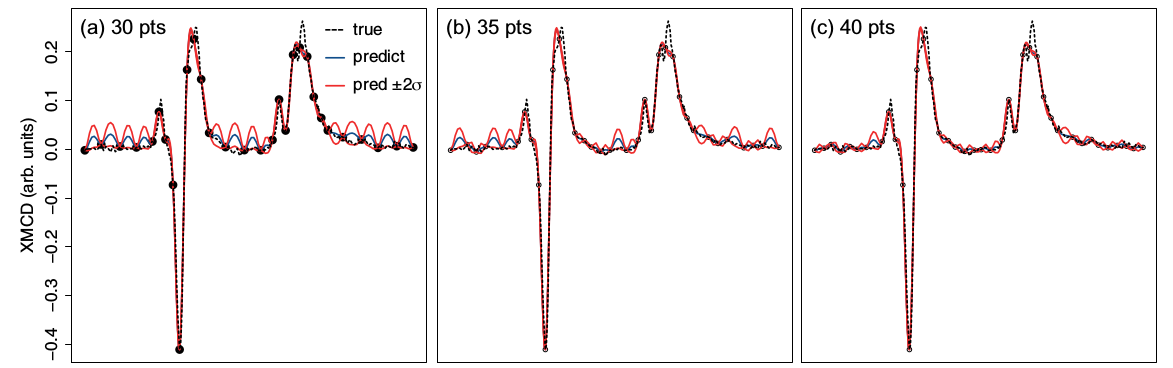
\includegraphics[width=0.75\textwidth]{Materials/Sepctroscopy1.png}
\caption{示意图}
\end{figure}
图中,Black Dashed:真实的光谱数据; Blue Solid: GP的预测结果; Black filled circles: 用到的数据点; Red Sold: 预测波形的$\pm 2\sigma$置信区间.
\end{frame}

\begin{frame}
\frametitle{背景}
为了得到材料的光谱图进行分析,

\textbf{传统的做法}:
\begin{itemize}
\item 利用大量不同波长Wavelength或能量(Energy)的X射线对材料进行扫描(Point by Point Scanning),得到满足信噪比要求的\textbf{光谱图}\footnote{与Wavelength或Energy成非线性关系}。
\item 实验测量(Measurement)与分析(Analysis)是分离的
\end{itemize}
\begin{figure}[!b]
\centering
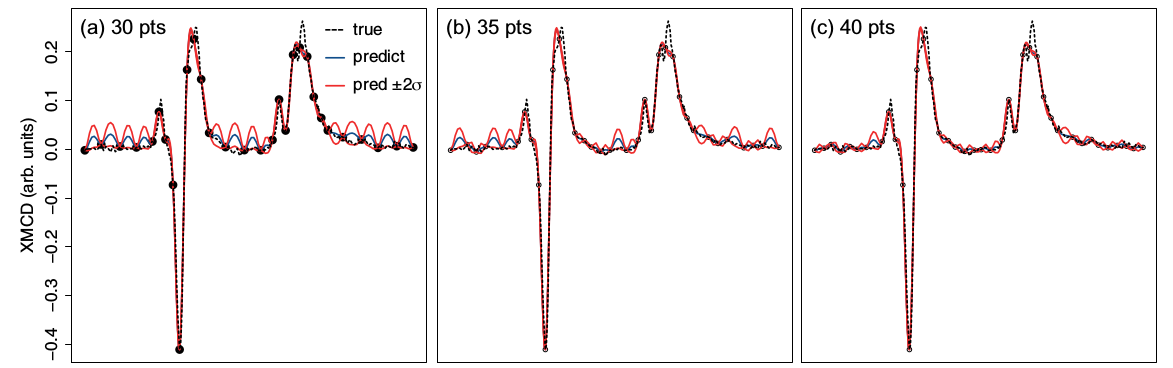
\includegraphics[width=0.75\textwidth]{Materials/Sepctroscopy1.png}
\end{figure}

\end{frame}

\begin{frame}
\frametitle{实验手段对比}
为了得到材料的光谱图进行分析,

\textbf{传统的做法}:
\begin{itemize}
\item 利用大量不同波长Wavelength或能量(Energy)的X射线对材料进行扫描(Point by Point Scanning),得到满足信噪比要求的\textbf{光谱图}\footnote{与Wavelength或Energy成非线性关系}。
\item 实验测量(Measurement)与分析(Analysis)是分离的
\end{itemize}
%\pause
\textbf{论文提出的解决思路}:
\begin{itemize}
\item 初始化
\begin{itemize}
\item 在$S_m M_{4,5}$吸收谱的Pre-edge、Post-edge之间均匀采样(30个)
\item 在峰值附近采样
\end{itemize}
\item 采样新的数据点 \\
若初始化中得到的数据点不满足需要,则重新进行采样。
\item 利用GP对离散的采样点进行插值回归,得到连续的图谱
\end{itemize}

\end{frame}

\begin{frame}
\frametitle{新的测量方式}
\begin{columns}
\column{0.55\textwidth}
\begin{figure}
\centering
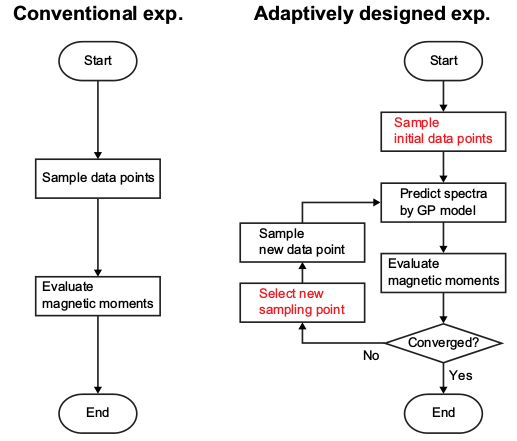
\includegraphics[width=0.75\textwidth]{Materials/Spectroscopy2.png}
\caption{对比图}
\end{figure}
注意,判断算法的有效性是通过计算磁矩来确定的,而不是预测完全正确的光谱。

\column{0.5\textwidth}
与传统的测量方式相比,优势在于:
\begin{itemize}
\item 依靠高效的采样、GP回归策略,降低了所需的数据采样点。Initial data points只需要30个
\end{itemize}

采样策略同样对结果具有较大的影响。在Select new sampling point中用的策略:
\begin{itemize}
\item 最大方差采样
\item 随机采样
\item 以方差为权重的随机采样
\end{itemize}
\end{columns}
\end{frame}

\begin{frame}
\frametitle{几种采样类型的实际表现}
\begin{figure}
\centering
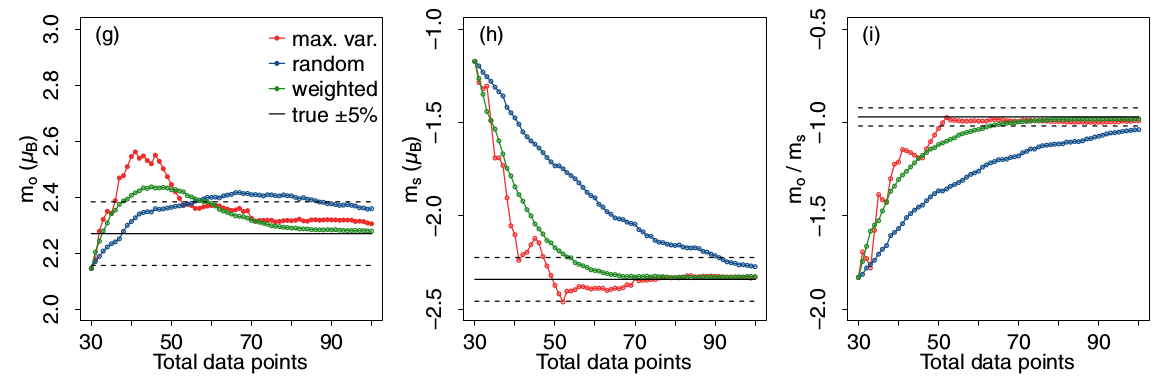
\includegraphics[width=0.75\textwidth]{Materials/Samples1.png}
\caption{三类采样方式的实验效果}
\end{figure}
可以看出,\textbf{最大方差采样}效果最好,收敛速度最快。
\end{frame}

\begin{frame}
\frametitle{具体算法}
\begin{itemize}
\item 实验设置
\begin{itemize}
\item $S_mC_{o_5}$的XMCD(X-ray Magnetic Circular Dichroism)以及XAS(X-ray Absorption Spectrum)光谱
\item $F_eC_o$合金的上述光谱
\end{itemize}

\item Magneto-optical sum rules \\
对XMCD与XAS光谱应用Magneto-optical Sum Rules可以得到材料的磁距:Orbital Magnetic Moment($m_o$), Spin Magnetic Moment($m_s$)
\item GP产生连续光谱

\end{itemize}
\end{frame}

\begin{frame}
\frametitle{GP回归算法--模型}
\begin{itemize}
\item 模型  \\
构建输入与输出的关系。
\begin{displaymath}
y(x_i) = \mu + z(x_i), i \in {1, \ldots, n}
\end{displaymath}
其中,$x_i$为Energy(或波长),$y(x_i)$为对应的输出,即光谱。在高斯模型中,$z(x_i)$为正态分布:$z(x_i) \sim Norm_{x}(0, \sigma^2R_{ij})$,$R_{ij}$为高斯相关函数$R_{ij}=exp(-\theta|x_i - x_j|^2)$,最终得到Y符合多元高斯分布:
\begin{displaymath}
Y \sim Norm_Y( \boldsymbol{1}_n\mu, \sigma^2R)
\end{displaymath}

\item 学习\\
利用最大似然法确定模型中的参数$\theta$。

\item 推理\\
对于新得到的数据进行预测。

\end{itemize}
\end{frame}

\begin{frame}
\frametitle{GP回归算法--学习与推理}
\begin{itemize}
\item 学习\\
最大化似然法计算$\hat{\theta}$:
\begin{displaymath}
\hat{\theta} = argmin_{\theta} \; log[Pr(Y | X, \theta)]
\end{displaymath}

\item 推理\\
利用学习得到的$\hat{\theta}$,进行预测:
\begin{displaymath}
\hat{y}(x^*) = \hat{\mu} + r^TR^{-1}(Y-\boldsymbol{1}_n\hat{\mu})
\end{displaymath}

\end{itemize}
\end{frame}

\begin{frame}
\frametitle{优势与不足}
\begin{figure}
\centering
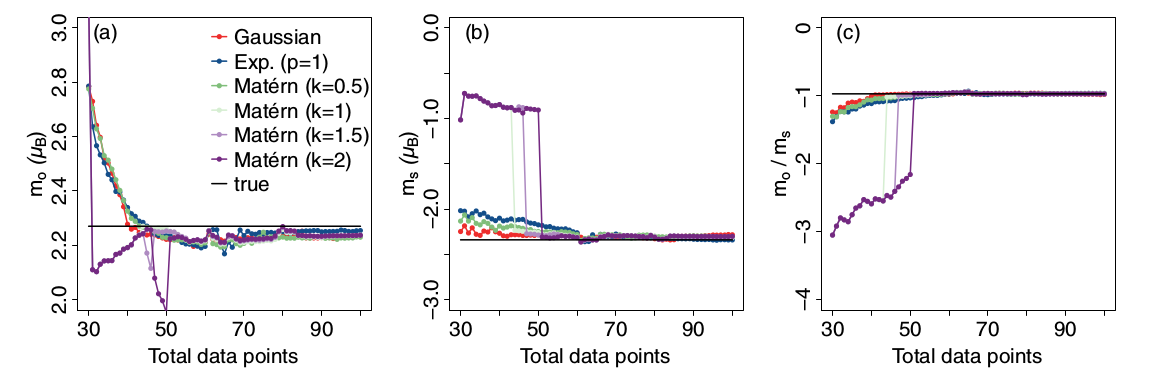
\includegraphics[width=0.6\textwidth]{Materials/Results1.png}
\end{figure}

\begin{itemize}
\item 优势
\begin{itemize}
\item 通过在少量Energy得到的离散光谱点,利用GP回归算法得到连续的光谱图,然后进行磁矩分析,提高了实验效率
\item 在进行GP计算时,可以进一步借助一些近似算法来加快计算。
\end{itemize}
\item 不足
\begin{itemize}
\item 预测的光谱图与实际光谱图之间还是有差距,只不过满足了后续的磁矩分析要求的精度
\item 可进一步提高收敛速度
\end{itemize}
\end{itemize}

\end{frame}

\subsection{基于机器学习算法分析材料的相变}

\begin{frame}
\tableofcontents[
sectionstyle=show/show,
subsectionstyle=show/share/hide,
currentsubsection,
]
\end{frame}

\begin{frame}
\frametitle{摘要(目的)}
\begin{itemize}
\item 利用机器学习算法,在序参量\footnote{相变临界点的一个物理量,如温度、电压等}未知的情况下,得到材料的纳米尺度的结构相变图,以及临界区(Critical Regimes)及相界(Phase Boundaries)等。
\end{itemize}
\begin{figure}[!b]
\centering
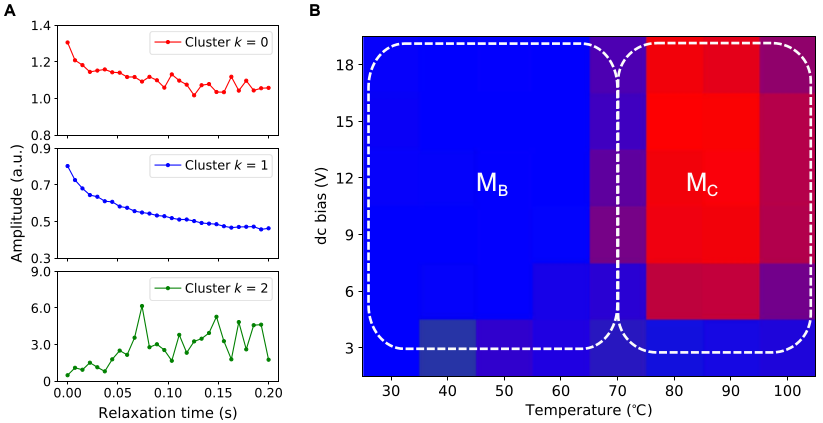
\includegraphics[width=0.5\textwidth]{Materials/Phase1.png}
\caption{示意图}
\end{figure}
\end{frame}

\begin{frame}
\frametitle{背景}
\textbf{相变(Phase Transition)}:
\begin{itemize}
\item 研究相变,有助于研究相变临界区发生的磁极系数(Susceptibility)的增强(Enhancement)
\item 相变可由序参数(Order parameter)表征
\item 对于纳米尺度的结构,序参数的确定是十分复杂的,无论是理论研究还是实验研究,均是如此
\item 可以利用机器学习自动生成特征(Feature)代替不可测量(Unmeasurable。或未知Unknown)的序参数
\end{itemize}
\textbf{测量装置}:
\begin{itemize}
\item Piezoresponce Force Microscopy(PFM),可以测量纳米尺度下Piezoresponce效应,序参数未知
\item 材料:PMN-27.5PT Crystals
\end{itemize}
\end{frame}

\begin{frame}
\frametitle{实验步骤}
\begin{itemize}
\item \textbf{开始}:\\
测量2D Ising System的参数:Ferromagnetic(逆磁性)-to-Paramagnetic(顺磁性)的相变、比热容。自由度(DoF)已知
\item \textbf{施加电场}\\
对应于不同的电场强度,测量若干个“Relaxation Curves”:$A = {A_1, A_2, \ldots, A_n}, A_i \in R^d$, n=100为Curves的数量,d=28为维度、等于测量次数(number of time steps)。此时DoF未知
\item \textbf{改变温度}\\
对应每一个电场强度,测试八种不同的温度。所以共:100 * 8个松弛曲线
\item \textbf{利用K-means对上述Curves进行聚类} \\
类别数$k$由人为输入,试验中,$k=3$
\end{itemize}
\end{frame}


\begin{frame}
\frametitle{用到的机器学习算法--PCA}
试验中,共设置了n=100个不同的电场强度,对应于每一个电场强度是维度d=28的一维向量,表征在d个不同时间点测量得到的数据;同时,试验中进一步设置了8个不同的温度。因此,得到的输入数据为一个$800 \times 28$的矩阵。

\begin{itemize}
\item PCA \\
对输入矩阵$M$进行SVD分解
\begin{displaymath}
M = USV^T
\end{displaymath}
矩阵V中每一列为M的奇异向量,其对应的奇异值降序排列,在分析实验数据时,基于V的前若干列(主成份)进行分析相变情况。示意图见下页。
\end{itemize}
\end{frame}

\begin{frame}
\frametitle{实验结果--PCA}
\begin{figure}
\centering
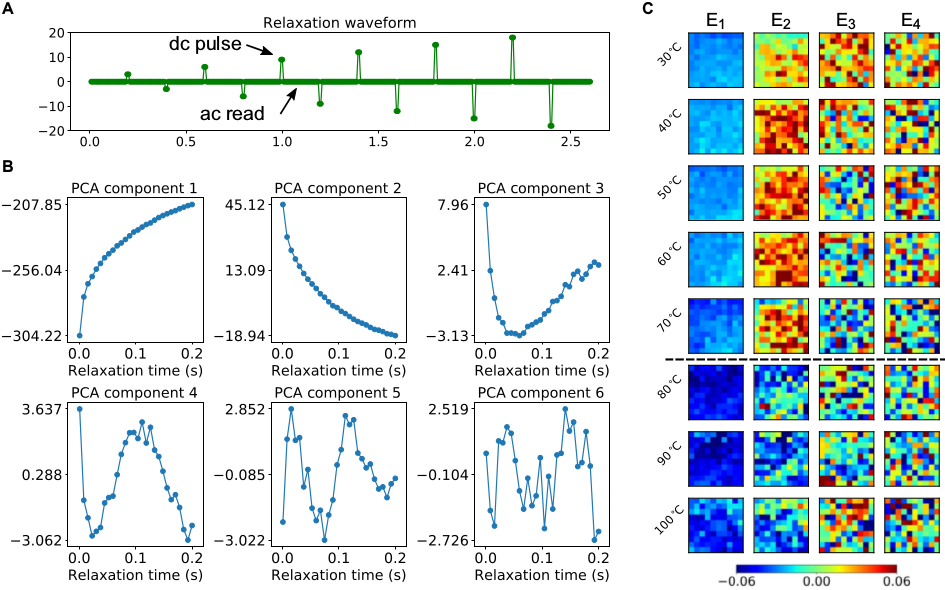
\includegraphics[width=0.7\textwidth]{Materials/PCA1.png}
\caption{PCA结果}
\end{figure}
从图c中可以看出,前两个最大的奇异值在$70^{\circ}C$与$80^{\circ}C$之间变化较大,意味着相变发生。
\end{frame}

\begin{frame}
\frametitle{用到的机器学习算法--K Means}
\textbf{PCA算法的缺点}:
\begin{itemize}
\item 缺少物理解释
\item 在辨别不同相(Phase)时,特征值较小但比较重要的成份被忽略
\end{itemize}

\textbf{改进(使用K-means)}:
\begin{displaymath}
arg min \sum_{j=1}^{k}\sum_{A\in S_j}\parallel A - \mu_j \parallel^2
\end{displaymath}
其中,A为输入的28维向量,代表一个测量曲线,$\mu_j$为第$j$类的中心,$S_j$为属于第$j$类的向量的集合。
\begin{itemize}
\item 使用所有数据,而不像PCA那样仅使用少数数据
\item 每一类中心对应与材料的一种“相”(Phase)
\end{itemize}

\end{frame}

\begin{frame}
\frametitle{实验结果--K Means}
\begin{figure}
\centering
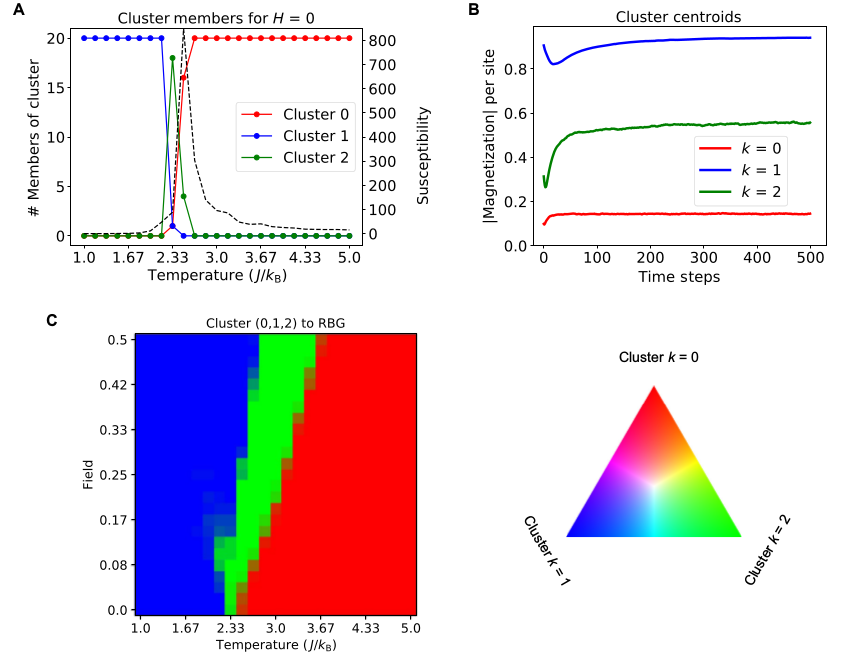
\includegraphics[width=0.7\textwidth]{Materials/KMeans.png}
\caption{K-Means结果}
\end{figure}

\end{frame}

\begin{frame}
\frametitle{优势与不足}
\begin{itemize}
\item \textbf{优势}:
\begin{itemize}
\item 基于实验数据,可自动生成相变图,而无需复杂的计算序参数
\item 算法较简单
\end{itemize}
\item \textbf{不足}:
\begin{itemize}
\item 需要人为输入聚类数,即$k$
\end{itemize}
 
\end{itemize}

\end{frame}

\subsection{小结}

\begin{frame}
\tableofcontents[
sectionstyle=show/show,
subsectionstyle=show/share/hide,
currentsubsection,
]
\end{frame}

\begin{frame}
\frametitle{机器学习在材料相变、光谱分析中的应用两篇论文小结}
这两个实验:
\begin{itemize}
\item \textbf{体现了在两个方面的应用}:
\begin{itemize}
\item 改进实验手段(如降低光谱图生成过程中所需的数据点(Scanning points))
\item 帮助实验结果的数据分析
\end{itemize}
\item \textbf{具有以下特点}:
\begin{itemize}
\item 用到的机器学习算法都比较简单,如K-Means, PCA, 高斯回归等
\item 提高了实验效率
\end{itemize}
\end{itemize}
\end{frame}

\section{未知目标检测}

\subsection{研究现状}

\begin{frame}
\frametitle{未知目标检测科学问题}
未知目标检测与以下几个研究方向比较接近:

\begin{itemize}
\item \textbf{One-shot/Few-shot Learning} \\
少样本学习。

训练集中存在少量的目标类型样本。

\item \textbf{Zero-shot Learning (ZSL)} \\
零样本学习。

训练集中不存在目标类型样本,测试集中不存在已知类型样本。

\item Open-set Recognition \\
最符合我们的目的。测试集里面同时存在已知与未知目标类型。

\item Life-long Machine learning

\end{itemize}


\end{frame}

\begin{frame}
\frametitle{相关算法}

\begin{itemize}
\item 基于高层特征----属性的学习算法

\item 迁移学习

\item 增量学习(Incremental Learning)

\item RNN Memory Based

\item 度量学习

\item 元学习(Meta Learning)

\item Learning to learn

\item 关系网络(Relation Network)

等。

\end{itemize}

\end{frame}

\subsection{未知目标检测与Zero-shot Learning}

\begin{frame}
\frametitle{未知目标检测与Zero-shot Learning}
文章\cite{Recent2017}中对Zero-shot Learning (ZSL)的解释:
\begin{quote}
{ \footnotesize
ZSL aims to recognize an object instance from a new category \textbf{never seen} before.

The task of identifying classes without any observed data is called ZSL.

** The ZSL can be considered a type of life-long learning. $\ldots$ This ability is termed "learning to learn".
}
\end{quote}
文章\cite{Unseen2018}中对未知目标检测的叙述:
\begin{quote}
$\ldots$ This situation calls for open-world classification or simply open classification which can classify those examples from the seen classes and also detect/reject examples from unseen or novel classes.
\end{quote}

\end{frame}

\begin{frame}
\frametitle{Recent Advances in ZSL}
\begin{columns}
\column{0.5\textwidth}
Recent Advances in Zero-shot Recognition.
\begin{figure}
\centering
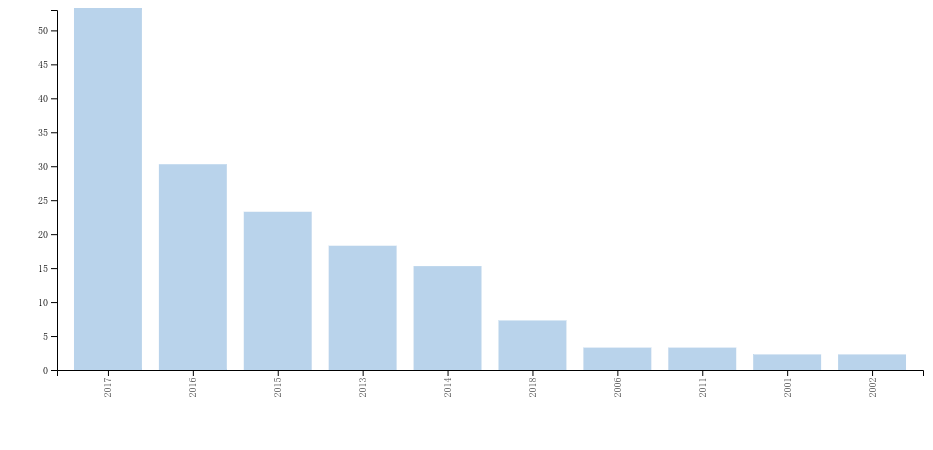
\includegraphics[width=0.9\textwidth]{Materials/visualization.jpg}
\caption{相关文章数,关键字:Zero shot learning}
\end{figure}

\column{0.65\textwidth}
\begin{itemize}
\item 基本框架\\
借助语义的帮助,进行识别。步骤:
\begin{itemize}
\item 基于Embedding Model建立目标(包括已知与未知)与语义之间的映射关系
\item 基于Recognition模块判断目标是否为未知
\end{itemize}
文章分别对上述两个步骤进行了综述。\cite{Discrimintive2018}与\cite{ZSR2018}(CVPR2018 Oral)基本符合这个框架。

\end{itemize}

\end{columns}
\end{frame}

\subsection{Unseen Class Discovery}
\begin{frame}
\frametitle{未知目标检测}
Unseen Class Discovery in Open-world classification
\begin{figure}
\centering
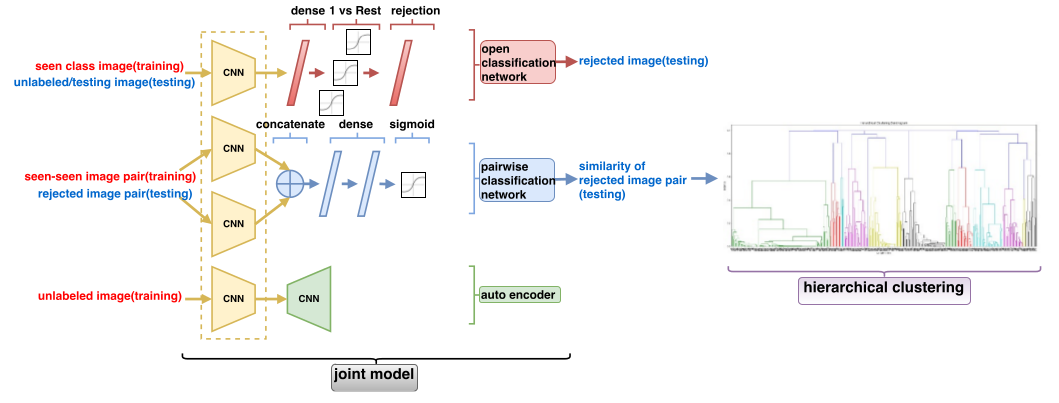
\includegraphics[width=0.75\textwidth]{Materials/Unseen1.png}
\caption{示意图}
\end{figure}
由四部分组成:
Open Classification Network(OCN), Pairwise Classification Network(PCN), Auto-encoder, Hierarchical clustering
\end{frame}

\begin{frame}
\frametitle{算法细节}
\begin{itemize}
\item OCN: \\
结构:一层卷积 + 最大池化层 + 两层全连接 + ReLU + 1-vs-rest layer\\
主要通过1-vs-rest层实现未知目标检测,以m个sigmoid函数 + 阈值的方式实现
\item PCN: \\
判断一对目标是否属于同一类
\item Auto-encoder \\
对未知目标生成表示
\item Hierarchical clustering\\
对未知目标(Rejected object)进行聚类学习。
\end{itemize}
\end{frame}

\subsection{相关文献}
%\begin{frame}%[allowframebreaks]    % % Work ! ! !
%\frametitle<presentation>{References}
%\nocite{*}
%\bibliographystyle{abbrv}
%\bibliography{ReferencesB}
%\end{frame}

\begin{frame}[allowframebreaks]
  \frametitle<presentation>{References}    
  \begin{thebibliography}{10}    
  \beamertemplatearticlebibitems
  \bibitem{Recent2017}
    Yanwei Fu, etc.
    \newblock {\em Recent Advances in Zero-shot Recognition}.
    \newblock zrXiv:1710.04837, 2017.
  \beamertemplatearticlebibitems
  \bibitem{Unseen2018}
    Lei Shu, Hu Xu, Bing Liu.
    \newblock {\em Unseen Class Discovery in Open-world Classification}.
    \newblock arXiv:1801.05609, 2018.
  \beamertemplatearticlebibitems
  \bibitem{ZSR2018}
   Xiaolong Wang, Yufei Ye, Abhinav Gupta.
   \newblock {\em Zero-shot Recognition via Semantic Embedding and Knowledge Graphs}.
   \newblock arXiv:1803.08035, 2018.
 \beamertemplatearticlebibitems
    \bibitem{Discrimintive2018}
      Yan Li, etc.
      \newblock {\em Discriminative Learning of Latent Features for Zero-Shot Recognition}.
      \newblock arXiv:1803.06731, 2018.
 \beamertemplatebookbibitems
    \bibitem{lifelong2016}
      Chen Zhiyuan, Bing Liu.
      \newblock {\em Lifelong machine learning}.
      \newblock Synthesis Lectures on Artificial Intelligence and Machine Learning, 2016.
  \end{thebibliography}
\end{frame}

\begin{frame}
\frametitle{研究课题组}
付彦伟、
\begin{itemize}
\item 付彦伟, 复旦大学大数据学院
\item Lampter, 
\item Liu Bing, 伊利诺伊大学洛杉矶分校
\end{itemize}

\end{frame}

\begin{frame}[plain]

{
\Large
\bfseries
\begin{center}
\color{orange}请各位\color{green}老师、同学\color{blue}批评指正!
\end{center}
}

\end{frame}

\end{document}
